\documentclass[10pt]{article}

\usepackage[utf8x]{inputenc}
\usepackage[english,italian]{babel}
\usepackage{graphicx} 
\usepackage{booktabs}
\usepackage{caption}
\usepackage{textgreek}
\usepackage{tabularx}
\usepackage{amsmath,amssymb,stackengine}
\usepackage{authblk}
\usepackage{xcolor}


\usepackage{geometry} % to change the page dimensions
\geometry{a4paper} % or letterpaper (US) or a5paper or....
% \geometry{margin=2in} % for example, change the margins to 2 inches all round
% \geometry{landscape} % set up the page for landscape
%   read geometry.pdf for detailed page layout information

\usepackage{graphicx} % support the \includegraphics command and options

% \usepackage[parfill]{parskip} % Activate to begin paragraphs with an empty line rather than an indent

%%% PACKAGES
\usepackage{booktabs} % for much better looking tables
\usepackage{array} % for better arrays (eg matrices) in maths
\usepackage{paralist} % very flexible & customisable lists (eg. enumerate/itemize, etc.)
\usepackage{verbatim} % adds environment for commenting out blocks of text & for better verbatim
\usepackage{subfig} % make it possible to include more than one captioned figure/table in a single float
% These packages are all incorporated in the memoir class to one degree or another...

%%% HEADERS & FOOTERS
\usepackage{fancyhdr} % This should be set AFTER setting up the page geometry
\pagestyle{fancy} % options: empty , plain , fancy
\renewcommand{\headrulewidth}{0pt} % customise the layout...
\lhead{}\chead{}\rhead{}
\lfoot{}\cfoot{\thepage}\rfoot{}

\usepackage{sectsty}
\allsectionsfont{\sffamily\mdseries\upshape} 

\usepackage[nottoc,notlof,notlot]{tocbibind}
\usepackage[titles,subfigure]{tocloft} 

\renewcommand{\cftsecfont}{\rmfamily\mdseries\upshape}
\renewcommand{\cftsecpagefont}{\rmfamily\mdseries\upshape} 
\newcommand*{\hham}{\mathcal{H}}
\newcommand*{\xx}{\vec{x}}
\newcommand*{\kk}{\vec{k}}
\newcommand*{\qq}{\vec{q}}
\newcommand*{\p}{\varphi}
\newcommand*{\zpart}{\mathcal{Z}}
\newcommand*{\w}{\Bigl}
\newcommand*{\lapint}{\int_{a-i\infty}^{a+i\infty}\frac{dz}{2\pi i}}

\definecolor{carmine}{rgb}{0.59, 0.0, 0.09}


\selectlanguage{english}

\title{{\bf Notes on ecosystems stability}}

\author{Onofrio Mazzarisi}

%\affil{{\it Max Planck Institute for Mathematics in the Sciences, Leipzig, Germany}}

\begin{document}

\selectlanguage{english}

%\begin{abstract}
%\end{abstract}

\maketitle

\section{Complexity-stability regimes}
\label{sec: complexity-stability regimes}
In this section we describe how the relationship between complexity and stability
is shaped by dynamical properties of complex ecosystems.

Consider a competitive community of $S$ species
defined by the following dynamics for the population abundances
\begin{equation}
    \frac{dx_i}{dt}=x_i^{\alpha}-x_i^{\beta}\sum_{j}A_{ij}x_j^{\gamma} \, ,
\end{equation}
where the sum runs from $j=1$ to $j=S$ and the off-diagonal elements
of $A$ are extracted from a distribution
with mean $\mu>0$ and standard deviation $\sigma$ while $A_{ii}=1/K^{\beta+\gamma-\alpha}$, $\forall i$,
and $K$ is the (uniform) carrying capacity.
If the equilibrium is feasible it formally reads
\begin{equation}
    (x_i^*)^{\alpha-\beta} = \sum_{j}A_{ij}(x_j^*)^{\gamma} \, .
\end{equation}
The element of the jacobian for $j\neq i$ read
\begin{equation}
    J_{ij} = -\gamma x_i^{\beta}A_{ij}x_j^{\gamma} \, ,
\end{equation}
while the diagonal components read
\begin{equation}
    J_{ii} = \alpha x_i^{\alpha-1}-\beta x_i^{\beta-1}\sum_{j\neq i}A_{ij}x_j^{\gamma}
    - (\beta+\gamma)A_{ii}x_i^{\beta+\gamma} \, .
\end{equation}

In the case of uniform interactions ($\sigma\to0$)
the species population are all equal and the equilibrium reads
\begin{equation}
    x^*=\left[\mu(S-1)+\frac{1}{K^{\beta+\gamma-\alpha}}\right]^{1/(\alpha-\beta-\gamma)} \, .
\end{equation}
The jacobian evaluated at equilibrium is
\begin{equation}
    J_{ij}\Big{|}_{x=x^*} = -\gamma \mu (x^*)^{\beta+\gamma-1} \, ,
\end{equation}
\begin{equation}
    J_{ii}\Big{|}_{x=x^*} = \alpha (x^*)^{\alpha-1}-\beta (x^*)^{\beta+\gamma-1}\mu(S-1)
                            -\frac{(\beta+\gamma)}{K^{\beta+\gamma-\alpha}}(x^*)^{\beta+\gamma-1}\, .
\end{equation}

The maximum eigenvalue $\lambda_{\textrm{max}}$ is $S-1$ degenerate and reads formally
\begin{equation}
    \lambda_{\textrm{max}} = J_{ii}\Big{|}_{x=x^*} - J_{ij}\Big{|}_{x=x^*} \, .
\end{equation}
The stability condition
\begin{equation}
    \lambda_{\textrm{max}} = \alpha (x^*)^{\alpha-1}-(x^*)^{\beta+\gamma-1}\left[\beta \mu(S-1)
    +\frac{(\beta+\gamma)}{K^{\beta+\gamma-\alpha}}-\gamma\mu\right]<0 \, ,
\end{equation}
can be written as
\begin{equation}
    \alpha (x^*)^{\alpha-\beta-\gamma}-\left[\beta \mu(S-1)
    +\frac{(\beta+\gamma)}{K^{\beta+\gamma-\alpha}}-\gamma\mu\right]<0 \, ,
\end{equation}
which, using the expression for $x^*$ and after some manipulations reads
\begin{equation}
    (S-1)(\beta-\alpha) > \frac{K^{\beta+\gamma-\alpha}\mu\gamma+\alpha-\beta-\gamma}{K^{\beta+\gamma-\alpha}\mu} \, .
\end{equation}
We have then three possibilities:
\begin{align}
    S &> 1 + \frac{K^{\beta+\gamma-\alpha}\mu\gamma+\alpha-\beta-\gamma}{K^{\beta+\gamma-\alpha}\mu(\beta-\alpha)} 
    &\textrm{if} \quad \alpha<\beta \, , \\
    S &< 1 + \frac{K^{\beta+\gamma-\alpha}\mu\gamma+\alpha-\beta-\gamma}{K^{\beta+\gamma-\alpha}\mu(\beta-\alpha)} 
    &\textrm{if} \quad \alpha>\beta \, , \\
    \mu &< \frac{1}{K^{\gamma}} &\textrm{if} \quad \alpha=\beta \, .
\end{align}
A series of comments is in order. 
\begin{itemize}
    \item Depending on $\alpha$ and $\beta$ we have \textit{two
    regimes}: one in which increasing $S$ enhances stability ($\alpha<\beta$) and 
    one in which it hinders stability ($\alpha>\beta$).
    Notably this is independent from $\gamma$, indicating that only the interplay between
    the density dependence of the contribution of a species to the interactions and
    the density dependence of its production term that is (qualitatively) relevant; 
    and not the form of the contribution of the competitors to the interactions.
    \item The critical case ($\alpha=\beta$) recovers the usual GLV result
    for $\gamma=1$ and generalizes it for generic $\gamma$.
    \item For $K\to\infty$ and $\beta=1=\gamma$ we obtain
    \begin{equation}
        S=1+\frac{1}{1-\alpha} \, .
    \end{equation}
\end{itemize}
For symmetry reasons, it is probably sensible to consider 
models with $\gamma=\beta$,
leaving the potential asymmetry of the competitive interaction between two species
to the coefficient $A_{ij}$.

One can therefore identify two different regimes (complexity hinders stability (May) and 
complexity increases stability)
characterized by the dynamical response of the population with respect to their density
encoded in the exponents $\alpha$ and $\beta$, resepctively associated
to production and losses. The GLV case $\alpha=\beta$ is right in the middle for uniform
interactions ($\sigma\to0$) and falls into the May regime otherwise ($\sigma\neq0$). 

\section{On sublinear production}
\label{sec: On sublinear production}
Observations point towards sublinear production scaling
with respect to the population biomass density. 
This observations may refer to
dynamical production or to the equilibrium production observed
across a biomass gradient.

In this section we discuss how, although dynamical sublinear production
does not generally leads to sublinear production across a biomass
gradient, it might be necessary for sublinear scaling across a biomass gradient.

Let us focus on a single population example to calrify ideas.
Consider a production function of the form
\begin{equation}
    g(x) = r x^\alpha \, ,
\label{eq: production}
\end{equation}
where $x$ is the abundance of the population, $\alpha\leq1$
specify the intensity of sublinear dynamical scaling (linear when $\alpha=1$) 
and $r$ is the parameter that allows to move across a gradient.
Consider then a loss term of the form
\begin{equation}
    l(x) = z x^\beta \, .
\end{equation} 
The evolution equaiton for the population is 
\begin{equation}
    \frac{dx}{dt} = g(x) - l(x) = r x^\alpha - z x^\beta \, ,
    \label{eq: single}
\end{equation} 
which reduces to logistic growth for $\alpha=1$ and $\beta=2$.
The equilibrium is given by
\begin{equation}
    x^* = \left(\frac{r}{z}\right)^{1/(\beta-\alpha)} \, ,
\label{eq: equilibrium single}
\end{equation}
and the stability condition is given by
\begin{equation}
    \frac{d\left[g(x)-l(x)\right]}{dx}\bigg|_{x=x^*} < 0 \, ,
\end{equation}
which leads, after some calculations, to the condition
\begin{equation}
    \alpha<\beta \, ,
\end{equation}
independent from $r$ and $z$.

The equilibrium production scales, at varying growth rate $r$,
as $g(x^*)=z(x^*)^\beta$ as can be noted by Eq.~(\ref{eq: equilibrium single})
for $r$ and then substituting it in the defining Eq.~(\ref{eq: production})
or simply by considering the dynamical equation at stationarity.
Notice that, if $z$ is varied instead, the exponent
of dynamical and across-gradient production coincide.

In summary, for an environmental change that amount to a change in $r$, 
the production across a gradient 
scales as $(x^*)^\beta$. In order for
the stationary solution to be stable an exponent $\alpha<\beta$
for the dynamical produciton is needed.
Therefore, in order to have sublinear $g(x^*)$ across a gradient,
we need $\alpha<\beta<1$.
If the increment of the equilibrium density is due to decreasing $x$,
equilibrium and dynamical production scale in the same way and in order to
have sublinear $g(x^*)$ we need $\alpha<1$ with $\alpha<\beta$ for stability
but no constraint on $\beta$. Either way we need $\alpha<1$.

\section{Cavity solution for sublinear growth}
\label{sec: cavity solution}
In this section we derive the cavity solution which is used in the main text.
(Refs.~\cite{Bunin2017,Barbier18,Barbier17,Advani2018,Cui2020,Roy2019})

Let us consider the dynamics of the abundances $x_i$ of $S$ species
\begin{equation}
    \frac{d x_i}{dt} = r_ix_i^k - z_ix_i - x_i\sum_{j\neq i}A_{ij}x_j\, ,
    \label{eq: full system}
\end{equation}
where the entries of the interaction matrix $A_{ij}$
and are independently distributed with average $\mu$ and standard deviation $\sigma$
and $r_i$ and $z_i$ are respectively growth rates 
extracted from distributions $P(r)$ and $P(z)$. 

Let us first give an informal argument to develop intuition and show
a clean connection between the initial system and the approximation
obtained through the cavity method~\footnote{Notice that the simple 
connection we portray here is possible in the specific settings
we consider but not in general, in particular the absence of correlation
between off-diagonal elements of the matrix simplifies things.}.
If we decompose the interaction matrix as $A_{ij}=\mu + \sigma a_{ij}$,
with $a_{ij}\sim \mathcal{N}(0,1)$, the steady-state solutions $x_i^*$ of
Eq.~(\ref{eq: full system}) are defined by
\begin{equation}
    0 = r_i(x_i^*)^k - x_i^*\left(z_i + \mu\sum_{j\neq i}x_j^* + \sigma\sum_{j\neq i}a_{ij}x_j^*\right)\, .
\end{equation}
For large $S$ we can write 
\begin{equation}
    \sum_{j\neq i}x_j^* \simeq S\langle x^* \rangle\, ,
\end{equation}
where $\langle x^* \rangle$ is the first moment of the steady state distribution,
the second sum in the above equation is more problematic to simplify 
because in principle $a_{ij}$ and $x_j$ are correlated variables.
The cavity method allows to rigorously and quantitatively justify 
the fact that, for a large community (i.e. large $S$) with random interactions,
a single species, say $x_i$, does not have a strong impact
on the full steady-state distribution. 
Therefore one does not do much wrong in
considering the steady-state abundances $x_j^*$, for $j\neq i$,
statistically independent from the paths from species $i$, $a_{ij}$.
We can then invoke Central Limit Theorem (CLT) and write
\begin{equation}
    \sum_{j\neq i}a_{ij}x_j^*\simeq \sqrt{S\langle (x^*)^2 \rangle}\eta \, ,
\end{equation}
$\eta$ is a standard normal random variable, i.e. $\eta\sim\mathcal N (0,1)$.
We have 
\begin{equation}
    0 = r_i(x_i^*)^k - x_i^*\left(z_i + \mu S\langle x^* \rangle + \sigma\sqrt{S\langle (x^*)^2 \rangle}\eta\right)\, ,
\end{equation}
which, by noticing that the species $i$ is statistically equivalent to each other species
in the community, therefore dropping the pedix, 
and solving for the representative abundance $x^*$ we obtain the cavity solution
\begin{equation}
    x^* = \left(\frac{z + \mu S \langle x^* \rangle + \sigma \sqrt{S\langle (x^*)^2\rangle} \eta}
    {r}\right)^{1/(k-1)} \, .
    \label{eq: cavity solution}
\end{equation}

Before discussing this result, let us give a slightly more formal justification.
The conceptual steps in the construction of the result (see, e.g., \cite{Barbier17}) can be stated as:
\begin{itemize}
    \item Start with a community of $S-1$ species.
    \item Add a species and consider only linear response of the initial community.
    \item Consider non-linear feedback on the added species and find steady-state.
    \item Notice that each species is statistically equivalent to the added species.
\end{itemize}
Starting from Eq.~(\ref{eq: full system}) and using the decomposition 
of $A_{ij}=\mu+\sigma a_{ij}$ we can write, for large $S$,
the steady state equation for an initial system of $S-1$ species as
\begin{equation}
    0 = r_i(x_i^*)^k - x_i^*\left(z_i + \mu S\langle x^* \rangle + \sigma\sum_{j\neq i}a_{ij}x_j^*\right)\, ,
\end{equation}
with $i \in \{1,\dots, S-1\}$. Introducing the species $S$
causes the following change
\begin{equation}
    0 = r_i(x_i^*)^k - x_i^*\left(z_i + \mu S\langle x^* \rangle + \sigma\sum_{j\neq i}a_{ij}x_j^* +\sigma a_{iS}x_S^*\right)\, ,
\end{equation}
which can be interpret as a perturbation to the mortality $z_i$.
Defining now the susceptibilities
\begin{equation}
    \chi_{ij} := \frac{dx_i}{dz_j} \, ,
\end{equation}
we can express the steady-state abundance of the species in the augmented
community as a first-order Taylor expansion around the values of the one
with $S-1$ species
\begin{equation}
    x_i^* \simeq x_{i \setminus S}^* - \sigma\sum_{j=1}^{S-1}\chi_{ij}a_{jS}x_S^*\, ,
\end{equation}
where we now denote by $x_{i \setminus S}^*$ the steady-state abundance
in the community in absence of species $S$.
The steady-state equation for species $S$ reads
\begin{equation}
    0 = r_S(x_S^*)^k - x_S^*\left(z_S + \mu S\langle x^* \rangle + \sigma\sum_{i=1}^{S-1}a_{Si}x_i^*\right)\, ,
\end{equation}
where, using the Taylor expansion for $x_i^*$, the interaction term can be written as
\begin{equation}
    \sum_{i=1}^{S-1}a_{Si}x_i^* = \sum_{i=1}^{S-1}a_{Si}x_{i\setminus S}^* - 
    \sigma\sum_{i=1}^{S-1}\sum_{j=1}^{S-1}a_{Si}a_{jS}\chi_{ij}x_S^* \, .
\end{equation}
The second term on the r.h.s. of the above equation vanishes because
$a_{Si}$ and $a_{jS}$ are independent variables, both for $j\neq i$ and $j=i$
in our setting. The first term is a product of two independent variable
and therefore, by means of CLT, we can write
\begin{equation}
    \sum_{i = 1}^{S-1}a_{Si}x_i^*\simeq \sqrt{S\langle (x^*)^2 \rangle}\eta \, .
\end{equation}
Finally, considering that species $S$ is statistically equivalent to
every other species we obtain again the cavity solution~(\ref{eq: cavity solution})
\begin{equation}
    x^* = \left(\frac{z + \mu S \langle x^* \rangle + \sigma \sqrt{S\langle (x^*)^2\rangle} \eta}
    {r}\right)^{1/(k-1)} \, ,
\end{equation}
where $\langle x^*\rangle$ and $\langle (x^*)^2\rangle$ are 
the first two moments of the abundance distribution, 
$\eta\sim\mathcal N (0,1)$ and $r$ and $z$ are distributed according to $P(r)$
and $P(z)$.
The steady-state probability distribution function for $x^*$, $P(x^*)$,
can be obtained, explicitly in some cases, 
through the pushforward of the distribution of $\eta$, $r$ and $z$ and
the fraction of survival species $\phi$ and the first two moment
have can then be self-consistently computed as
\begin{align}
    \phi&= \int_0^{\infty}dx^* \ P(x^*)\, , \nonumber \\
    \langle x^*\rangle&=\frac{1}{\phi}\int_0^{\infty}dx^* \ x^*P(x^*) \, , \label{eq: self-consistenty}\\
    \langle (x^*)^2\rangle&=\frac{1}{\phi}\int_0^{\infty}dx^* \ (x^*)^2 P(x^*) \, . \nonumber
\end{align}

In the case of a unique $r$ for every species in the community and vanishing $z$
the distribution reads
\begin{equation}
    P(x^*)=\frac{(1-k)|x^*|^{k-2}}{\sqrt{2\pi \sigma^2 S\langle (x^*)^2 \rangle/r^2}}
    \exp{\left\{-\frac{\left[(x^*)^{k-1}-\mu S\langle x^*\rangle/r\right]^2}{2\sigma^2S\langle (x^*)^2 \rangle/r^2}\right\}} \, .
    \label{eq: species dist unique r}
\end{equation}
We can't formally solve the self-consistent equations~(\ref{eq: self-consistenty})
because the first and second moment of  for this distribution diverges.
A similiar problem is encountered in Ref.~\cite{Cui2020}
in the context of consumer-resource models for the cavity calculations of
the distribution of the resources which is, \textit{mutatis mutandis}, 
equivalent of our case for $k=0$.

Following~\cite{Cui2020} and assuming the fluctuations in the numerator in Eq.~(\ref{eq: cavity solution})
are small, i.e. $\sigma \sqrt{S\langle (x^*)^2\rangle}\ll \mu S \langle x^* \rangle$,
we Taylor expand to the first-order the cavity solution obtaining
\begin{equation}
    x^* = \left(\frac{ \mu S \langle x^* \rangle}{r}\right)^{1/(k-1)} -
    \frac{1}{1-k}\left(\frac{ \mu S \langle x^* \rangle}{r}\right)^{(2-k)/(k-1)}\sigma \sqrt{S\langle (x^*)^2\rangle}\eta \, ,
\end{equation}
which is a gaussian variable, truncated in 0 to respect
non-negativity constraint, with mean
\begin{equation}
    \langle x^* \rangle = \left(\frac{ \mu S \langle x^* \rangle}{r}\right)^{1/(k-1)} \, ,
\end{equation}
and standard deviation
\begin{equation}
    \sqrt{\langle (x^*)^2 \rangle - \langle x^* \rangle^2} =
    \frac{1}{1-k}\left(\frac{ \mu S \langle x^* \rangle}{r}\right)^{(2-k)/(k-1)}\sigma \sqrt{S\langle (x^*)^2\rangle} \, .
\end{equation}

In this approximation we can solve analytically 
the self consistency equations for the first to moment of the
distribution as functions of the parameters, namely 
\begin{equation}
    \langle x^* \rangle = \left(\frac{ \mu S}{r}\right)^{1/(k-2)} \, ,
    \label{eq: SM first moment}
\end{equation}
and
\begin{equation}
    \langle (x^*)^2 \rangle = \frac{ \langle x^* \rangle^2}
    {\left[1-\left(\frac{1}{1-k}\right)^2\langle x^* \rangle^{2(2-k)}
    \sigma^2S\right]} \, .
    \label{eq: SM second moment}
\end{equation}
We can therefore use this gaussian approximation to describe the
species distribution.

For practical purposes, and in order to more closely recover
results from simulations we can also solve numerically the self-consistent
equations~(\ref{eq: self-consistenty}) using a large
upper cut off $x_{\textrm{up}}$ which we checked can be widely varied
and gives consistent results.
In Fig.~\ref{fig: SM cavity + gauss} we report comparisons
of the cavity solution~(\ref{eq: species dist unique r}) 
obtained solving numerically the self-consistent equations
and the gaussian approximation.

\begin{figure}[h!]
    \centering
    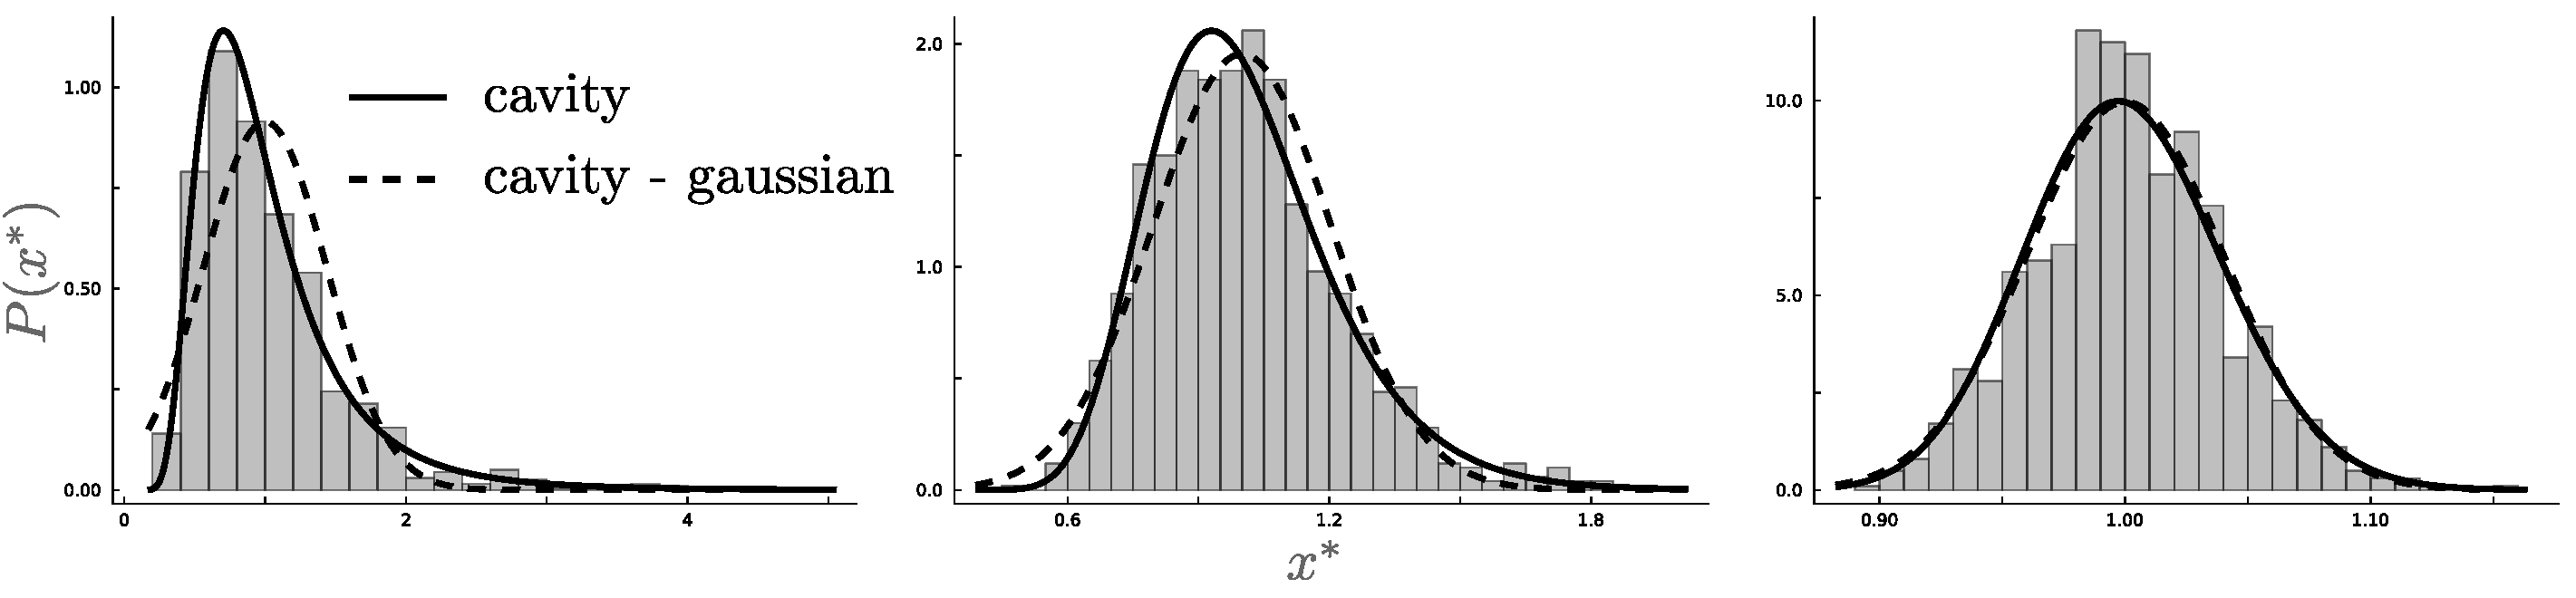
\includegraphics[width=1\textwidth]{fig/SM-cavity+gaussian.pdf}
    \caption{Cavity solution in Eq.~(\ref{eq: species dist unique r}) (solid line) 
    with the moment numerically self-consistently computed using the
    full distribution and the gaussian approximation (dashed line)
    are compared with simulation for a system 
    of $S=10^3$ species with
    $r=1$, $\mu=10^{-3}$, $k=3/4$ and $\sigma=\mu/10$ (left),
    $\sigma=\mu/20$ (center) and $\sigma=\mu/100$ (right).}
    \label{fig: SM cavity + gauss}
\end{figure}

\subsubsection{Stability condition}

Ahmadian \emph{et al.}~\cite{ahmadianProperties2015} consider large matrices of the form $M + LJR$, where $M$,  $L$ and $R$ are deterministic matrices, and $J$ is a random matrix with i.i.d. coefficients with zero mean and variance $\sigma^2$. Generalizing the classical `circular law', they show that the spectrum of such matrices is contained withing the region of the complex plane defined by 
\begin{equation}
    \textrm{Tr}[(M_\zeta M_\zeta^\dagger)^{-1}]\geq 1/\sigma^2 \quad \textrm{where}\ M_\zeta = L^{-1}(\zeta I - M)R^{-1}, 
\end{equation}
where $\textrm{Tr}$ denotes the trace, dagger the Hermitian conjugate, and $\zeta\in\mathbb{C}$. In the special case where $L$, $R$ and $M$ are diagonal, this condition reduces to
\begin{equation}
    \sum_{i=1}^S\frac{(L_{i}R_{i})^2}{ \vert \zeta - M_{i}\vert^2 }\geq 1/\sigma^2
\end{equation}
for matrices of size $S$. 

Following Stone~\cite{stoneFeasibility2018}, we now apply this result to generalize the stability condition to random interactions $A_{ij}$. From \eqref{community-matrix} we can write the community matrix as
\begin{equation}
    C^* = -\textrm{diag}(\mathbf x^*)[A + \textrm{diag}(\mathbf r  g'( \mathbf x^*))]\,
\end{equation}
where the product of vectors is understood component-wise. Denoting $\mathbf{1}$ the rank-one matrix with all entries equal to $1$, we can write $A = \mu \mathbf{1} - \mu I + J$ with $J$ as above. For the spectral properties of interest to us, relying on rank-one perturbation theory (see Ref.~\cite{stoneFeasibility2018}),
we can consider $A = - \mu I + J$, hence $C^*$ has the form $M + LJR$ with  
$L = -\textrm{diag}(\mathbf x^*)$, $R = I$ and $M = \textrm{diag}(\mathbf x^*)[\mu I + \textrm{diag}(\mathbf r g'(\mathbf x^*))]$. Thus, we have that the eigenvalues of the community matrix $C^*$ must lie within the domain 
\begin{equation}
    \sum_{i=1}^S\, \frac{(x_i^*)^2}{\vert \zeta -x_i^*[\mu + r_ig'(x_i^*)]\vert ^2}\geq 1/\sigma^2. 
    \label{eq: SM spectral domain}
\end{equation} 
The equation above is used in the main text to plot the spectral support of the eigenvalues in the complex plane.
This domain first touches the right half-plane at $\zeta = 0$, hence stability of $C^*$ requires   
\begin{equation}\label{random-stability}
    \sum_{i=1}^S\, [\mu + r_ig'(x_i^*)]^{-2}< \sigma^{-2}. 
\end{equation}

In the logistic model, we have $g'(x^*_i) = -1/K_i$, hence \eqref{random-stability} becomes $\sum_i (\mu - r_i/K_i)^{-2} < \sigma^{-2}$. When growth rates and carrying capacities are all equal, this is just the May condition $\sigma\sqrt{S} + \mu < r/K$, interpreted as stating that interaction strength $(\mu, \sigma)$ and diversity $S$ must be small compared to self-regulation $r/K$ to allow for stable coexistence.
In terms of scaled variables $\sigma\sqrt{S}$ and $\mu S$ instability
sets in for $\sigma\sqrt{S} + \mu S / S =  r/K$ and in the limit of
$S\to\infty$ the stability line for GLV in the scaled 
parameter space is given by 
\begin{equation}
    \sigma\sqrt{S} = r/K \, ,
\end{equation}

By contrast, in the sublinear model (defined by $g(x) = (x/x_0)^{k-1}$), we have $g'(x) = (k-1) x^{k-2}/x_0^{k-1}$, hence \eqref{random-stability} reads
\begin{equation}
    \sum_{i=1}^S\, [\mu - (1-k) r_i (x_i^*)^{k-2}/x_0^{k-1}]^{-2}< \sigma^{-2} \, .
\end{equation} 
Making use of the cavity solution $P(x^*)$ obtained in sec. \ref{cavity}
for equal $r$ for every species and vanishing $z$,
we can write this condition as 
\begin{equation}
    S \int dx^* \ P( x^*)[\mu - (1-k) r (x^*)^{k-2}/x_0^{k-1}]^{-2}< \sigma^{-2} \, .
\end{equation}
The stability line in the scaled parameter space 
can be obtained from the above expression
\begin{equation}
    \sigma\sqrt{S} = \left\{\int dx^* \ P( x^*)[\mu S / S - (1-k) r (x^*)^{k-2}/x_0^{k-1}]^{-2}\right\}^{-1/2} \, .
\end{equation}
In the limit $S\to \infty$ and noticing that $P(x^*)$ depend
on $S$ only through $\sigma\sqrt{S}$ and $\mu S$ we finally obtain
\begin{equation}
    \sigma\sqrt{S} = \left\{\int dx^* \ P( x^*)[(1-k) r (x^*)^{k-2}/x_0^{k-1}]^{-2}\right\}^{-1/2} \, .
\end{equation}

In order to obtain the stability line we solve, 
for a given $S$ and given $\mu$,
the set of self-consistency equations plus the stability condition
numerically, either by using the full cavity solution, Eq.~(\ref{eq: species dist unique r}), or the gaussian approximation using the moments
in Eq.~(\ref{eq: SM first moment}) and Eq.~(\ref{eq: SM second moment})
\begin{align}
    \phi&= \int_0^{\infty}dx^* \ P(x^*)\, , \nonumber \\
    \langle x^*\rangle&=\frac{1}{\phi}\int_0^{\infty}dx^* \ x^*P(x^*) \, , \label{eq: self-consistenty}\\
    \langle (x^*)^2\rangle&=\frac{1}{\phi}\int_0^{\infty}dx^* \ (x^*)^2 P(x^*) \, , \nonumber \\
    \sigma\sqrt{S} &= \left\{\frac{1}{\phi}\int_0^{\infty} dx^* \ P( x^*)[(1-k) r (x^*)^{k-2}/x_0^{k-1}]^{-2}\right\}^{-1/2} \, . \nonumber
\end{align}
The results are plotted in Fig.~\ref{fig: SM stability cavity + gaussian}.

\begin{figure}[h!]
    \centering
    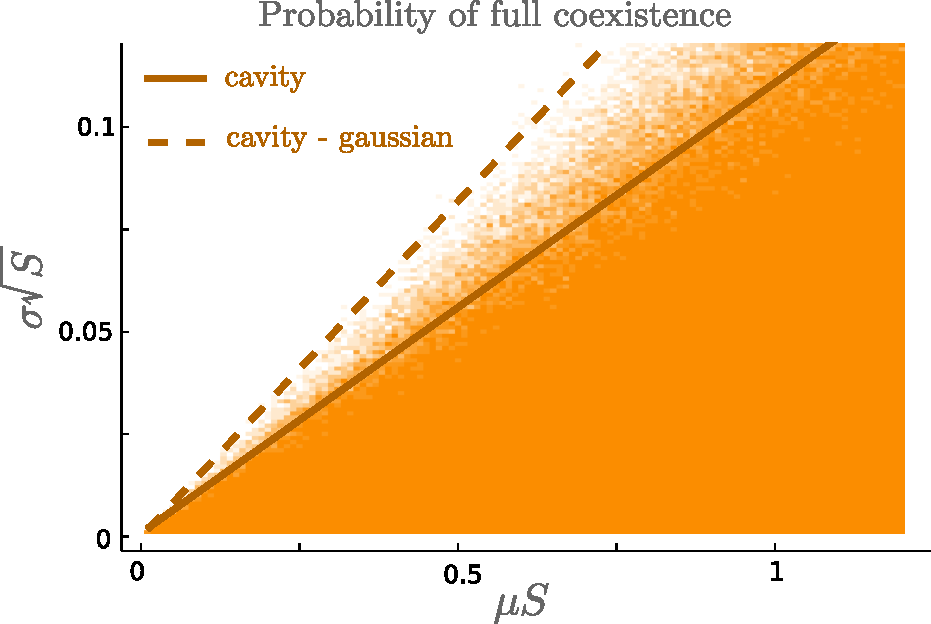
\includegraphics[width=.8\textwidth]{fig/SM-stability-cavity+gauss.pdf}
    \caption{Simulation showing probability of full coexistence, (from dark orange (probability 1)
    to white (probability 0)) compared with analytical estimation of the 
    stability threshold (solid line obtained 
    using the full cavity solution and
    the dashed line using the gaussian approximation).
    The number of species is kept fixed to $S=100$ and $\mu$ and $\sigma$
    are varied.}
    \label{fig: SM stability cavity + gaussian}
\end{figure}

\subsubsection{Extinction condition}
In this section we derive an expression to estimate the 
extinction threshold in parameter space. 
It can be obtained by means of the gaussian
approximation of the cavity solution.

We recall the definition for the first and
second moment of the distribution of $x$
\begin{equation}
    \langle x^* \rangle = \left(\frac{ \mu S}{rx_0^{1-k}}\right)^{1/(k-2)} \, ,
\end{equation}
and
\begin{equation}
    \langle (x^*)^2 \rangle = \frac{ \langle x^* \rangle^2}
    {\left[1-\left(\frac{1}{1-k}\right)^2\langle x^* \rangle^{2(2-k)}
    \sigma^2S\right]} \, ,
\end{equation}
where we explicitely wrote down the scale $x_0$ because
in the following we want to study both, the case
where the growth term is not modified below threshold
and when is set equal to zero causing every species below threshold
to go extinct.

First we approximate the second moment by expanding it
to the first order in the second addend in the denominator
\begin{equation}
    \langle (x^*)^2 \rangle \approx \langle x^* \rangle^2
    + \left(\frac{1}{1-k}\right)^2\langle x^* \rangle^{2(3-k)}\sigma^2 S \, ,
\end{equation}
so that the standard deviation can be written as
\begin{equation}
    \sqrt{\langle (x^*)^2 \rangle - \langle x^* \rangle^2} \equiv \textrm{std}(x^*)=
    \left(\frac{1}{1-k}\right)\langle x^* \rangle^{(3-k)}\sigma \sqrt{S} \, .
\label{eq: SM approx second moment}
\end{equation}

Now we want to write down the condition under which
the average minus a number $\nu$ of standard deviations
touches zero, or $x_0$ if the threshold is enforced.
Let us consider this latter more general case first.
The condition reads
\begin{equation}
    \langle x^*\rangle - \nu \ \textrm{std}(x^*)
    = x_0 \, ,
\label{eq: SM extinction condition}
\end{equation}
which, using Eq.~(\ref{eq: SM approx second moment}),
becomes
\begin{equation}
    \langle x^*\rangle - \nu\left(\frac{1}{1-k}\right)\langle x^* \rangle^{(3-k)}\sigma \sqrt{S}
    = x_0 \, .
\end{equation}
Substituting the expression for the average and solving for
$\sigma\sqrt{S}$, we finally obtain
\begin{equation}
    \sigma\sqrt{S} = \frac{1-k}{\nu}\left[\left(\frac{ \mu S}{rx_0^{1-k}}\right)
    -x_0\left(\frac{ \mu S}{rx_0^{1-k}}\right)^{(k-3)/(k-2)}\right] \, ,
    \label{eq: SM extinction line threshold}
\end{equation}
which reduces in the case where no condition is imposed in $x_0$
to the linear relation between the scaled parameters
$\sigma\sqrt{S}$ and $\mu S$
\begin{equation}
    \sigma\sqrt{S} = \left(\frac{1-k}{\nu rx_0^{1-k}}\right)\mu S \, .
    \label{eq: SM extinction line no threhsold}
\end{equation}

In order to avoid arbitrariness in the choice of $\nu$
we can estimate an $S$ dependent value which accounts for the fact
that the same equilibrium distribution but with more species
(therefore the same point in the $\sigma\sqrt{S} - \mu S$ plane for higher $S$)
implies a smaller sample minimum.
One way to make analytical progress is to find the value
$x_{\textrm{min}}$ for which the gaussian approximation for the distribution touches
$1/S$. There will be two points satisfying this conditions and we are interested
in the lower one. The rationale behind this is that in a community
of $S$ species, less then one, on average, will be below $x_{\textrm{min}}$.
We have 
\begin{equation}
    \frac{1}{\sqrt{2\pi\textrm{std}(x^*)^2}}
    \exp{\left[-\frac{(x_{\textrm{min}}-\langle x^* \rangle)^2}{2\textrm{std}(x^*)^2}\right]} = \frac{1}{S} \, ,
\end{equation}
which, solving for $x_{\textrm{min}}$, gives
\begin{equation}
    x_{\textrm{min}} = \langle x^* \rangle - \textrm{std}(x^*)\sqrt{2\ln\left(\frac{S}{\sqrt{2\pi\textrm{std}(x^*)^2}}\right)} \, .
\end{equation}
For large $S$ we can approximate the last equation by
\begin{equation}
    x_{\textrm{min}} = \langle x^* \rangle - \sqrt{2\ln S} \ \textrm{std}(x^*) \, ,
\end{equation}
from which we can read out our estimate for $\nu$, comparing with Eq.~(\ref{eq: SM extinction condition}),
i.e.
\begin{equation}
    \nu = \sqrt{2\ln S}\, .
\end{equation}

\begin{figure}[h!]
    \centering
    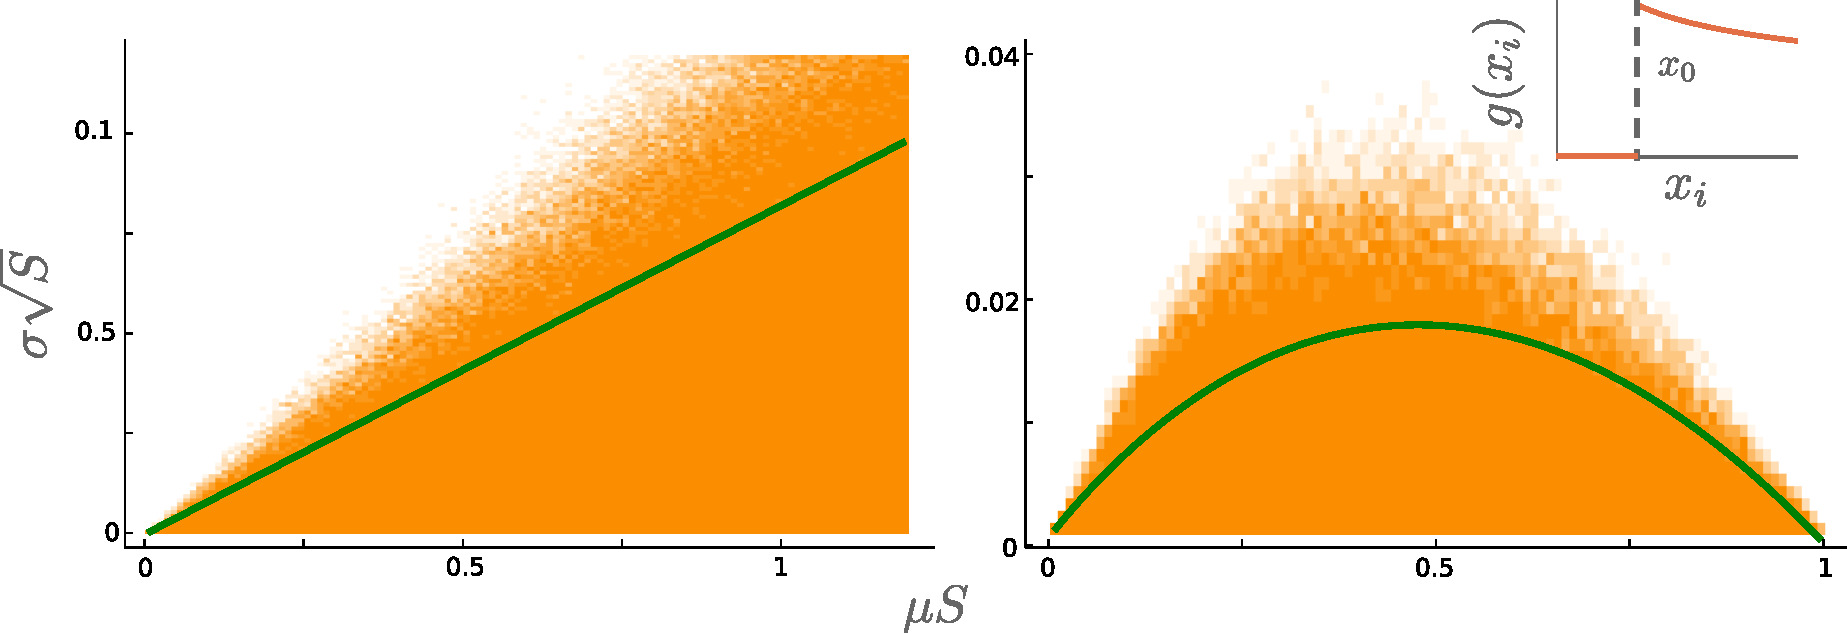
\includegraphics[width=1\textwidth]{fig/SM-extinction.pdf}
    \caption{Simulation showing probability of full coexistence, (from dark orange (probability 1)
    to white (probability 0)) compared with analytical estimation of the extinction threshold (green lines).
    In both panels the number of species is kept fixed to $S=100$ and $\mu$ and $\sigma$
    are varied, the left panel shows results for the case in which no threshold effect
    is enforced while the right panel report the case where growth is set to zero
    if the population of a species touches the threshold. The analytical lines are plotted
    from Eq.~(\ref{eq: SM extinction line no threhsold}) (left) and Eq.~(\ref{eq: SM extinction line threshold})
    (right) both with $\nu=\sqrt{2\ln S}$.}
    \label{fig: SM extinction threshold}
\end{figure}

In Fig.~(\ref{fig: SM extinction threshold}) the extinction threshold
is plotted against simulations for the case where no condition is imposed
at the threshold $x_0$ and the case where growth is set to zero below the threshold.

The same arguments apply to GLV, which, we recall, describes $S$ species evolving as
\begin{equation}
    \frac{dx_i}{dt} = r x_i(1-\frac{x_i}{K}) - x_i\sum_{j\neq i}A_{ij}x_j
\end{equation}
with $A_{ij}$ distributed with mean $\mu$ and standard deviation $\sigma$
and we assume here $r$ and $K$ equal for all species,
allowing to estimate the extinction threshold also in this case.

The equilibrium distribution obtained through the cavity method is
a truncated gaussian~[REFS] with average
\begin{equation}
    \langle x^* \rangle = \frac{K}{1+K\mu S/r} \, ,
\end{equation}
and standard deviation, written as a function of the average,
\begin{equation}
    \textrm{std}(x^*) = \frac{\sigma\sqrt{S}K\langle x^* \rangle}{\sqrt{1-\frac{K^2\sigma^2S}{r^2}}} \, ,
\end{equation}
plugging in the last two equations in the extinction 
threshold condition~(\ref{eq: SM extinction condition}), for $x_0=0$
leads to 
\begin{eqnarray}
    \sigma\sqrt{S} = \frac{r}{K\sqrt{\nu^2+1}} \, ,
\end{eqnarray}
which is an horizontal line in the parameter space 
lower then the stability condition $\sigma\sqrt{S}$ and recovers it for $\nu=0$.


\section{Model connection with data on productivity}
Our model is informed by macroecological observations
of biomass density production across major groups.
In this section we attempt a closer connection to the data.

We define our model in the following way
\begin{equation}
    \frac{d b_i}{dt} = \underbrace{r_ib_i\left(\frac{b_i}{b_0}\right)^{k -1}\theta(b_i-b_0)}_\text{Production}
     - \underbrace{b_i\sum_{j\neq i}A_{ij}b_j}_\text{Losses} \, ,
\end{equation}
where $k<1$
specify the intensity of sublinear dynamical scaling,
the entries of the interaction matrix $A_{ij}$
are randomly distributed with average $\mu$ and standard deviation $\sigma$,
the $r_i$ are growth rates extracted from a distribution
$P(r)$, the biomass density scale
$b_0$.
For the sake of clarity let us summarize the dimensionality of
the several terms involved in the model
\begin{equation}
    [b_i] = [b_0] =  \frac{\textrm{mass}}{\textrm{area}} \ ,
    \quad [r_i]=\frac{1}{\textrm{time}} \ , 
    \quad [A_{ij}]=\frac{\textrm{area}}{\textrm{mass}\times \textrm{time}} \ .
\end{equation}
The density biomass scale $b_0$ set the value at which the per capita
growth rate is $r_i$. When we want to consider this value the
maximum per capita growth rate for a given species we can
consider $b_0$ as the minimal biomass density for a given species
at which it is able to reproduce. 
In this case we can impose that there is no growth
for $b_i<b_0$ through a Heaviside function $\theta(b_i-b_0)$.

Next we connect the model with the average body mass $m$ of a community. 
The time scale of the problem are widely observed~\cite{Hatton2019}
to scale with the body mass with an exponent $-1/4$.
Therefore we assume that the average growth rate $\langle r \rangle$ for
a community and the average interaction $\mu$ scale with the average body mass
of the community to the $-1/4$, 
i.e. $\langle r\rangle\sim m^{-1/4}$ and $\langle \mu \rangle\sim m^{-1/4}$.
We have no reasons to assume a systematic variation of the ratio
$\mu/\sigma$ with respect to the mass.
We assume for simplicity that $b_0$ is species and mass independent. 
We may invoke an ecological argument
to justify this assumption, 
indeed the observed biomass densities across major group
have a mass independent lower bound (within two or three order of magnitude compared
with the astronomical difference of nearly 20 order of magnitude in body mass).
The population density scale for a given community of average mass
$m$, $n_0:=(b_0)/m$, is then assumed to be inversely proportional to the mass.

To compare this data with outcomes of the model
we proceede as follows. We characterize a community type
by an average mass, and therefore by an average growth rate $\langle r\rangle$,
then we solve the model for different communities with same average $r$ but
different $\mu$ and plot the resulting $\langle b^* \ g(b^*)\rangle$ vs 
$\langle b^*\rangle$. In this process we keep the coefficient 
of variation $\sigma/\mu$ constant.
We keep $S$ constant and vary $\mu$ in a range which scales
with $m$ in the same way that the average $r$ does across community type:
within a community type we plot results for communities with 
$\mu S\in(\langle r\rangle\mu_{\min}, \langle r\rangle\mu_{\max})$, with $\mu_{\min}$
and $\mu_{\max}$ possibly mass dependent but with $\mu_{\min}<1$ and $\mu_{\max}>1$.
In other words, in order to not introduce strong  biases towards specific
masses, within community type and for every community type,
we simulate different environment 
going from a $\mu$ which is 
less than $\langle r\rangle$ to one which is more than $\langle r\rangle$.
We can summarize the assumptions in the following way.
\\

\textbf{Assumptions}
\begin{itemize}
    \item $b_0$ is body mass independent
          and $n_0$ for a community is inversely proportional to the average
          body mass $m$ of the community.
    \item $ r \sim m^{-1/4}$ and characterize the typical growth rate
          of a community type with the typical body mass $m$.
    \item $\mu\sim m^{-1/4}$ for a given community type of average mass $m$.
    \item To explore ecological variation among communities
          of the same type we cosider different 
          $\mu S\in(r\mu_{\min}, r\mu_{\max})$
          with $\mu_{\min}<1$ and $\mu_{\max}>1$.
    \item the coefficient of variation $\mu/\sigma$ does not vary systematically
          both within and across community type.
    \item $k<1$, in particular, in orderd to closely recover the observed pattern, $k\simeq3/4$
\end{itemize}
Each point in Fig.~\ref{fig: SM production} 
correspond
to an entire community, with on the $x$ axis the average biomass
of the community $\langle b^* \rangle$ and on the $y$ axis the
average equilibrium production of the community 
$\langle b^* \ g(b^*)\rangle$. Within each community type the points follow
a scaling law with exponent aroun $3/4$.

\begin{figure}[h!]
    \centering
    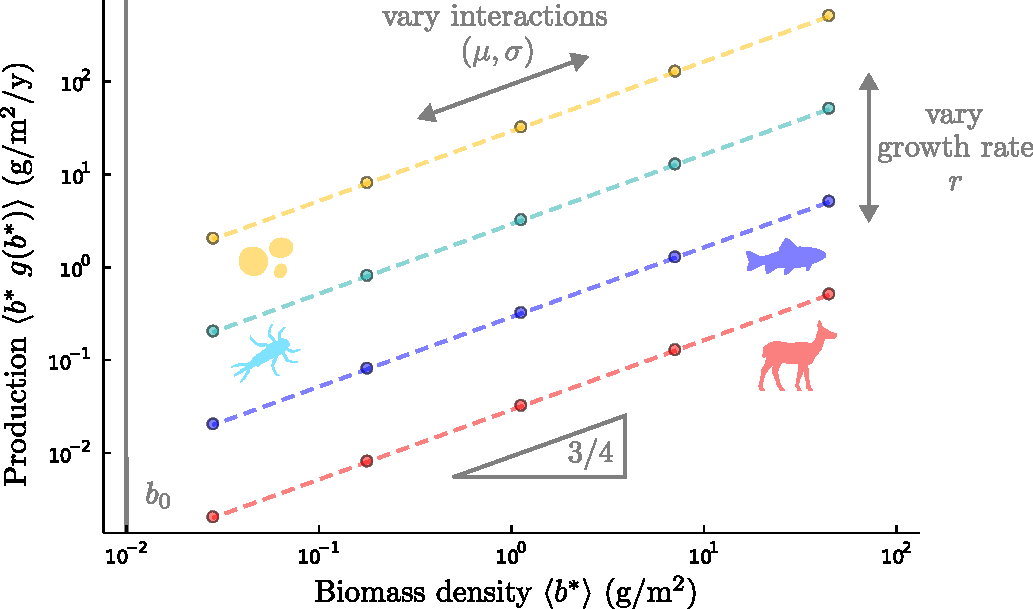
\includegraphics[width=.8\textwidth]{fig/SM-production.pdf}
    \caption{\textcolor{red}{Make figure with precise values of r} 
    Average equilibrium production $\langle b^* \ g(b^*)\rangle$ 
    plotted versus average equilibrium biomass density $\langle b^*\rangle$.
    Each dot represents simulations for a community of $S=50$ species, each color
    correspond to a specific growth rate value: $r=10^2$ yellow, $r=10$ light blue,
    $r = 1$ blue and $r= 10 ^{-1}$ red with the dimension of 1/y.
    The exponent in the growht rate
    is set as $k=3/4$ and the biomass scale is $b_0=10^{-2}$ (g/$\textrm{m}^2$),
    the different points within a color (i.e. same $r$) correspond to 
    $\mu S \in \{r10^2, r10, r, r^10^{-1}, r10^{-2}\}$. 
    We set everywhere the coefficient of variation $\sigma/\mu=0.7$.
    The dashed lines represent theoretical predictions from the
    cavity solution.}
    \label{fig: SM production}
\end{figure}

\subsection{Analytical prediction of average equilibrium production}
In order to compute how the average production changes with respect to 
the average biomass density in our context we can resosrt to the cavity
solution computed in the previous section which \textit{mutatis mutandis}
in terms of biomass density reads
\begin{equation}
    b^* = \left(\frac{\mu S \langle b^* \rangle + \sigma \sqrt{S\langle (b^*)^2\rangle} \eta}
    {r \ b_0^{1-k}}\right)^{1/(k-1)} \, .
    \label{eq: cavity solution biomass}
\end{equation}
At equilibrium we have
\begin{equation}
    b^*g(b^*)\equiv\underbrace{rb^*\left(\frac{b^*}{b_0}\right)^{k -1}}_\text{Production}
    = \underbrace{b^*(\mu S \langle b^* \rangle + \sigma \sqrt{S\langle (b^*)^2\rangle} \eta)}_\text{Losses} \, ,
\end{equation}
therefore
\begin{equation}
    \langle b^*g(b^*)\rangle =  \mu S \langle b^* \rangle^2 + 
    \sigma \sqrt{S\langle (b^*)^2\rangle} \langle b^*\eta\rangle \, .
    \label{eq: formal for production}
\end{equation}
Invoking the gaussian approximation we know that the average reads
\begin{equation}
    \langle b^*\rangle = \left(\frac{\mu S}{r \ b_0^{1-k}}\right)^{1/(k-2)} \, ,
\end{equation}
which, if inverted for $\mu S$, gives
\begin{equation}
    \mu S = r \ b_0^{1-k} \langle b^*\rangle^{k-2} \, ,
\end{equation}
which imply that the first term on the r.h.s. of Eq.~(\ref{eq: formal for production}) is
equal to $r \ b_0^{1-k}\langle b^* \rangle^k$.

The second term is more involved. By writing explicitely the expression for
$b^*$ it reads
\begin{align}
    \sigma \sqrt{S\langle (b^*)^2\rangle} \langle b^*\eta\rangle &= 
    \sigma \sqrt{S\langle (b^*)^2\rangle}
    \left\langle  \left(\frac{\mu S \langle b^* \rangle + \sigma \sqrt{S\langle (b^*)^2\rangle} \eta}
    {r \ b_0^{1-k}}\right)^{1/(k-1)} \eta\right\rangle \nonumber \, ,\\
    &= \sigma \sqrt{S\langle (b^*)^2\rangle} r^{1/(1-k)}b_0
    \left\langle  \frac{\eta}{(\mu S \langle b^* \rangle + 
    \sigma \sqrt{S\langle (b^*)^2\rangle} \eta)^{1/(1-k)}}\right\rangle \, .
\end{align}
The leading term in the denominator for large $S$ is
$(\mu S \langle b^* \rangle)^{1/(1-k)}$, which for $k=3/4$ is proportional
to $S^4$, while the others have a lower order dependence on $S$. Therefore
if we approximate the whole denominator by $(\mu S \langle b^* \rangle)^{1/(1-k)}$ 
and recall that $\langle \eta \rangle=0$ we can neglect this term
and approximate the average production as
\begin{equation}
    \langle b^*g(b^*)\rangle \simeq r \ b_0^{1-k}\langle b^*\rangle^k \, .
\end{equation}

\subsection{Note on the origin of sublinear growth}

Mechanistic justifications of the emergence
of sublinear dynamical growth at the coarse level of description
of the model studied in this work should be
sought after. However our results suggest
that mechanistic descriptions of community dynamics 
leading to an effective sublinear growth 
(or, more generally, to a relative change 
of production with respect of population abundance
lower than the relative change of losses,
see Sec.~\ref{sec: complexity-stability regimes})
will be qualitatively characterized by a positive
correlation beteween stability and complexity.

The macroecological data which inspired the model studied in this work
have mixed origin, some can be directely connected with
dynamical production and other are cross-ecosystem patterns.
More precise and systematic observations of the former 
and validation of the latter at the ecosystem level
with temporal data are needed 
(see Ref.~\cite{Barbier2021} for an example of a macroecologially motivated
model and subsequent discussion about within ecosystem validation).
\\\\

\textbf{Among the task that future theoretical work should aim at, we suggest}
\begin{itemize}
    \item Building a mechanistic understanding of the emergence
          of sublinear dynamical scaling from realistic models.
    \item Connecting the abundance prediction from community
          models with macroecological patterns related to abundance.
          In particular when we go from within community description
          to cross-community.
    \item Exploring in detail possibilities different from 
          sublinear dynamical scaling to explain cross-ecosystem 
          sublinear scaling and test indipendent predicrtions.
\end{itemize}

\textbf{Future urgent experimental and field research include}
\begin{itemize}
    \item Collecting temporal data within ecosystems and devise ways 
          to estimate the population abundance or density dependence
          on production.
    \item Extending the spectrum of data available in order to 
          further validate the evidence of sublinear production.
\end{itemize} 

\section{Macroecological laws}
In this section we compare macroecological patterns
with prediction of our model specifying in which way
we construct the observable to compare and under which assumptions
in addtion to the ones described in the construction of the model.

\subsection{Species abundance distribution}
The species abundance distribution distribution within a community
is often well fitted by a log-normal distribution.
In order to recover this pattern for the abundance density $n_i$ 
with our model we assume that
the growth rates $r_i$ follows a log-normal distribution.
\\

\textbf{Assumptions}
\begin{itemize}
    \item $\ln r\sim\mathcal{N} (\mu_r,\sigma_r)$.
\end{itemize}

\textbf{Predictions}
\begin{itemize}
    \item We predict that $n^*$ roughly follows a 
    log-normal distribution as well and, if we consider $k=3/4$,
    it has shape parameter 4 times larger than the one for $r$.
\end{itemize}

We can work out an exact calculation in the case of uniform interactions (i.e. $\sigma\to0$),
which works well also for small but finite $\sigma$.
In this case the cavity solution for $n^*$ (Eq.~(\ref{eq: cavity solution})) reads
\begin{equation}
    n^* = \left(\frac{\mu S \langle n^* \rangle}
    {r \ n_0^{1-k}}\right)^{1/(k-1)} \, ,
\end{equation}
where we recall that consider for simplicity that the scale $n_0$ is the same for all the species in
the community and set it to unity, $n_0=1$, in the following.

We can obtain the probability distribution for $n^*$ by pushing forward the one for $r$,
$P(n^*)=P(r(n^*))|dr/dn^*|$. Given that $r(n^*)$ reads
\begin{equation}
    r=\frac{(n^*)^{k-1}}{\mu S \langle n^* \rangle} \, ,
\end{equation}
and
\begin{equation}
    \left|\frac{dr}{dn^*}\right| = \frac{(1-k)(n^*)^{k-2}}{\mu S \langle n^* \rangle} \, ,
\end{equation}
we obtain that $n^*$ is as well a log-normal random variable
\begin{equation}
    \ln n^*\sim\mathcal N (\mu_{n^*}, \sigma_{n^*}) \, ,
    \label{eq: cavity for lognormal r}
\end{equation}
with 
\begin{align}
    \mu_{n^*} &= \frac{\mu_r - \ln{(\mu S \langle n^* \rangle)}}{(1-k)} \, , \\
    \sigma_{n^*} &= \frac{\sigma_r}{(1-k)} \, .
\end{align}
Notice that the scale parameter is amplified by a factor $1/(1-k)$, which in the
case of $k\simeq3/4$ correspond to a species abundance distribution four times
wider than the growth rate distribution.

In this case we only need to solve a self-consistent equation 
for the average $\langle n^* \rangle$ to complete the cavity solution.
This can be done analytically because the expression of the average
for a log-normal distribution is known
\begin{equation}
    \langle n^* \rangle = \exp{\left(\mu_{n^*}+\frac{\sigma_{n^*}^2}{2}\right)} \, ,
\end{equation}
and we have
\begin{equation}
    \langle n^* \rangle = (\mu S)^{(k-2)}
    \exp{\left[\frac{2\mu_r(1-k)+\sigma_r^2}{2(1-k)(2-k)}\right]} \, .
\end{equation}

In Fig.~\ref{fig: SM species abundance lognormal} the cavity results are compared with simulations showing
perfect agreement in the case $\sigma\to0$ (left panel)
and good agreement also in the case of finite $\sigma$ (right panel).

\begin{figure}[h!]
    \centering
    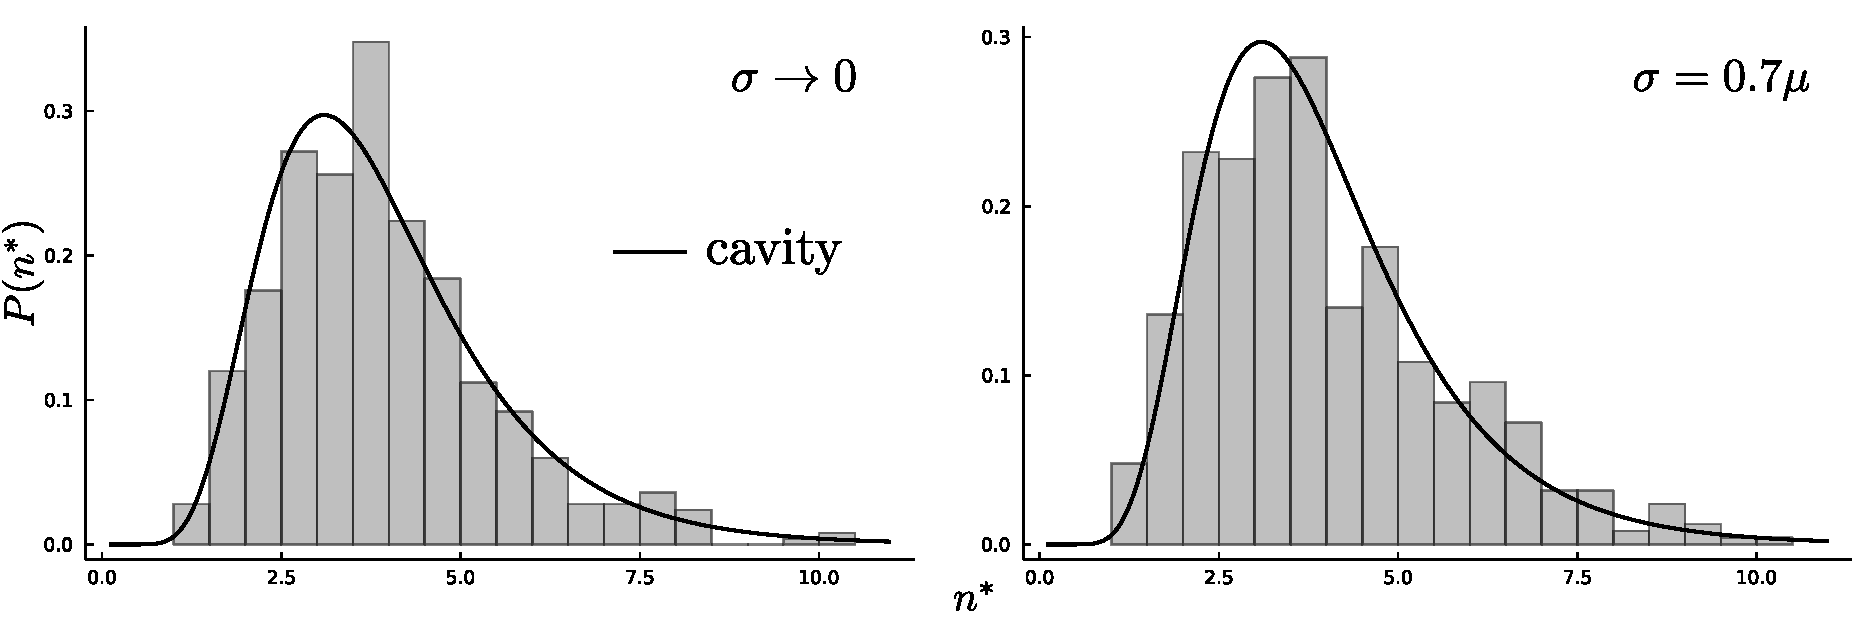
\includegraphics[width=1\textwidth]{fig/SM-species-abd.pdf}
    \caption{Cavity solution compared to simulations for log-normal distribution of growth rates $r$, 
    $\ln{P(r)}=\mathcal{N} (\mu_r,\sigma_r)$, with $\mu_r=1$ and $\sigma_r=1/10$
    and a pool of $S=500$ species with $\mu=10^{-3}$, $k=3/4$ and $\sigma\to0$ (left panel)
    while $\sigma=0.7\mu$ (right panel).}
    \label{fig: SM species abundance lognormal}
\end{figure}

In Fig.~\ref{fig: SM species abundance realistic} we report the abundance distributions
for the four community types as parametrized in the model construction (details in caption).

\begin{figure}[h!]
    \centering
    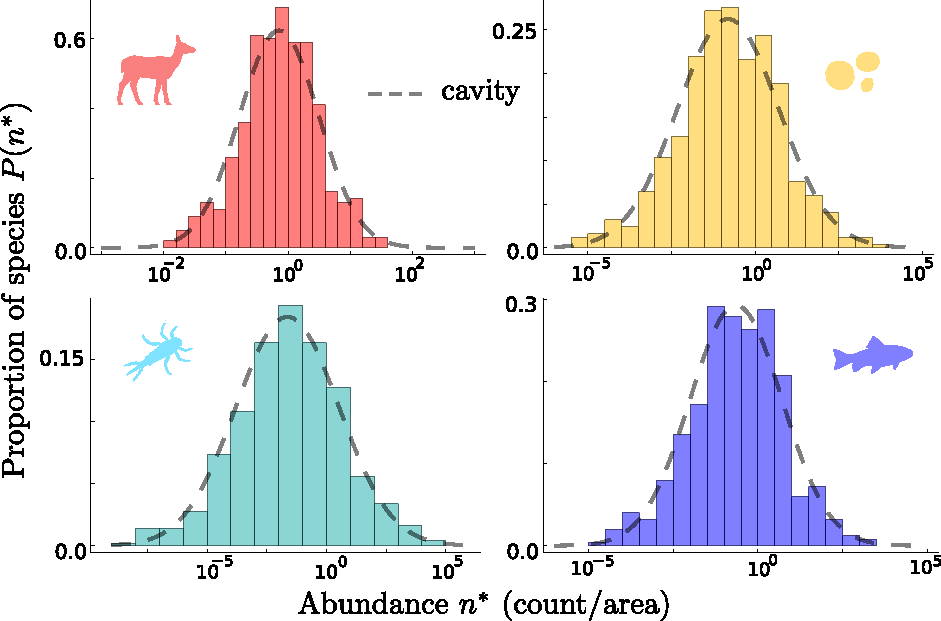
\includegraphics[width=.8\textwidth]{fig/SM-abundance-realistic2.pdf}
    \caption{Abundance distribution of species resulting from the dynamics
    for the four community types as parametrized in the model 
    construction see (Fig.~\ref{fig: SM production}), but with $S=500$ species
    to obtain better statistics. In particular, in every panels, 
    we set $\mu S = \langle r \rangle $ and $\sigma/\mu=0.7 $ and $r$
    is lognormally distributed with mode chose as 
    $\exp(\mu_r)=\langle r \rangle B_0^{1-k}$ specific for each color
    as per model construction and shape parameter $\sigma_r = 0.16$
    for red, 0.38 for blue, 0.54 for light blue and 0.34 for yellow.
    The dashed lines correspond to the cavity solution 
    in Eq.~(\ref{eq: cavity for lognormal r}) 
    which well compare with simulations.}
    \label{fig: SM species abundance realistic}
\end{figure}

\subsection{Mean-variance scaling}
The variance of fluctuations in biomass densities for time series
of different species scale with mean biomass density with an exponent
from $3/2$ to 2.
We consider again a log-normal distribution for $r$
and that the loss term of our model exhibits variation in mortality
(e.g. $\mu$ varies).
\\

\textbf{Assumptions}
\begin{itemize}
    \item $\ln r\sim\mathcal{N} (\mu_r,\sigma_r)$ (only needed for analytical results).
    \item $\mu$ varies (in the case of uniform $r$, the ratio $\mu/\sigma$ should be constant).
\end{itemize}

\textbf{Predictions}
\begin{itemize}
    \item Taylor's law.
\end{itemize}

We consider again the cavity result in the limit $\sigma\to0$
which, in the case of $\ln r\sim \mathcal N (\mu_r, \sigma_r)$,
gives $\ln b^*\sim\mathcal N (\mu_{b^*}, \sigma_{b^*})$ with
\begin{align}
    \mu_{b^*} &= \frac{\mu_r-\ln{(\mu S \langle b^* \rangle)}}{(1-k)} \, , \\
    \sigma_{b^*} &= \frac{\sigma_r}{(1-k)} \, .
\end{align}
By varying $\mu$ only the scale parameter $\mu_{b^*}$ is modified.
Therefore if we consider the mean and variace of the log-normal distribution
\begin{align}
    \langle b^* \rangle &= \exp{\left(\mu_{b^*}+\frac{\sigma_{b^*}^2}{2}\right)} \, , \\
    \textrm{var}(b^*)&=  
    \left(\exp[\sigma_{b^*}^2]-1\right)\exp{\left(2\mu_{b^*}+\sigma_{b^*}^2\right)}\, , \\
\end{align}
it is straightforward to realize that the mean is proportional to $\exp(\mu_{b^*})$, while
the variance to $\exp(2\mu_{b^*})$, therefore
\begin{equation}
    \textrm{var}(b^*) \propto  \langle b^* \rangle^2 \, ,
\end{equation}
i.e., Taylor's law.
In Fig.~\ref{fig: SM Taylor's law} we report a comparison 
with simulations with lognormally distributed $r$ and $\sigma\to0$, 
lognormally distribute $r$ and finite $\sigma=\mu/10$, to show
that the results hold in this case, and, even if in this case we don't have analytical results 
(\textcolor{red}{I manage to obtain one, to be added}),
also with uniform $r=1$ and 
finite $\sigma=\mu/10$.
\begin{figure}[h!]
    \centering
    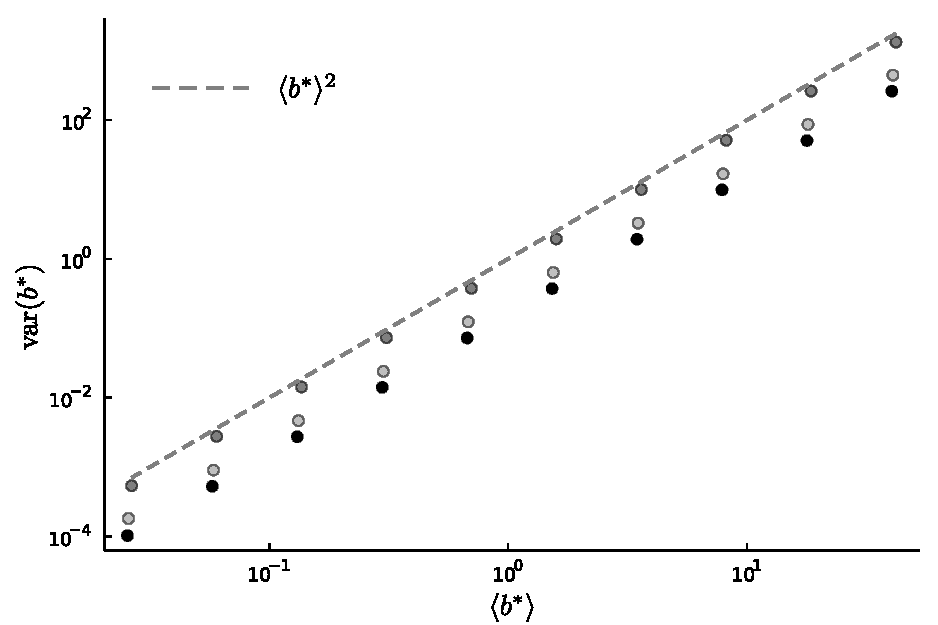
\includegraphics[width=.8\textwidth]{fig/SM-taylor-complete.pdf}
    \caption{Variance of the species biomass density distribution plotted against the mean,
    each dot is a community with a specific $\mu\in\{\langle r\rangle10^{-2},\langle r\rangle10^{2}\}$,    
    whith $S=10^3$, $k=3/4$ and black dots correspond to $\ln{P(r)}=\mathcal{N} (\mu_r,\sigma_r)$, 
    with $\mu_r=1$, $\sigma_r=1/10$ and $\sigma\to0$, dark gray to $\sigma=\mu/10$ with the same distribution
    for $r$ and light gray dots correspond to uniform $r=1$ and $\sigma=\mu/10$.}
    \label{fig: SM Taylor's law}
\end{figure}

In Fig.~\ref{fig: SM Taylor's law realistic} we report variance vs.
average for the communitites parametrized as in model construction (Fig.~\ref{fig: SM production}),
finding a good agreement with Taylor's law, see caption for details.

\begin{figure}[h!]
    \centering
    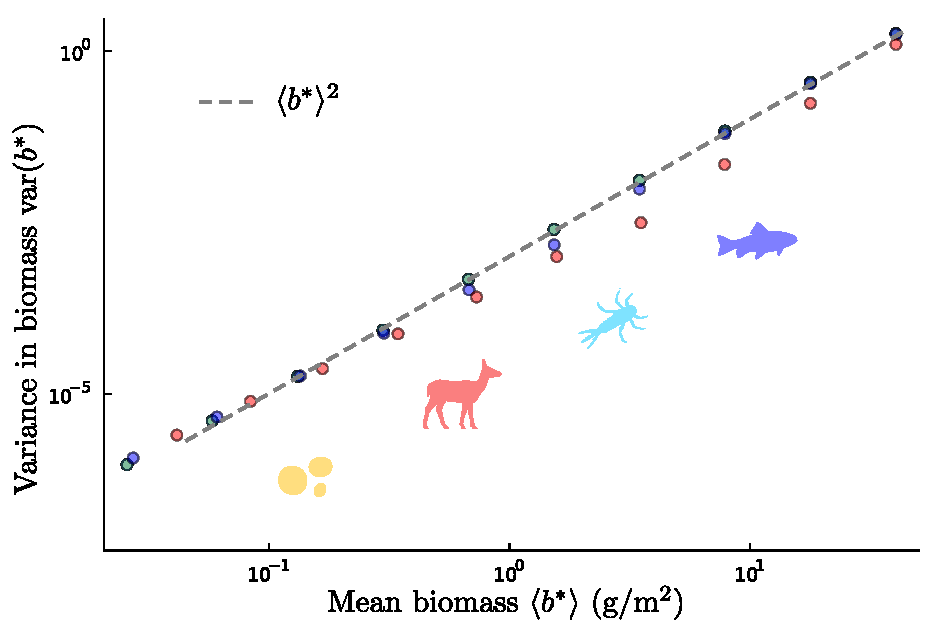
\includegraphics[width=.8\textwidth]{fig/SM-taylor-realistic.pdf}
    \caption{\textcolor{red}{Make figure with precise values of r} Variance of the species biomass density distribution plotted against the mean,
    each dot is a community is parametrized as in the model construction (see
    caption of Fig.~\ref{fig: SM production}).}
    \label{fig: SM Taylor's law realistic}
\end{figure}

\subsection{Size-density scaling}
The species-level relation of population density vs. body mass
is nearly inversely proportional across major groups.
By relying on no further assumptions then in those used
to connect the model with data on production we predict
a size-density scaling with exponent -1.

\textbf{Assumptions}
\begin{itemize}
    \item Same as for the connection of the model with data on production.
\end{itemize}

\textbf{Predictions}
\begin{itemize}
    \item Size-density scaling with exponent -1.
\end{itemize}

We start from the cavity solution for the equilibrium biomass density $b_0$
\begin{equation}
    b^* = \left(\frac{\mu S \langle b^* \rangle + \sigma \sqrt{S\langle (b^*)^2\rangle} \eta}
    {r \ b_0^{1-k}}\right)^{1/(k-1)} \, ,
\end{equation}
where we consider $r$ uniform and different for each community type as in the model
connection with data on production.
Each community is characterized by an average mass $m$, and, given that we consider
$\mu S \propto r$ (it varies in a range of two order of magnitude above and below $r$),
it cancels out with $r$ leaving no mass dependence.
Therefore the average numerical densities $\langle n^*\rangle$ 
of different community types will
be inversely proportional to their mass $m$ with a spread on the $y$ axes
due to different $(\mu, \sigma)$
\begin{equation}
    \langle n^*\rangle \sim m^{-1} \, .
\end{equation}
In Fig.~\ref{fig: SM size-density scaling} we report the average numerical density vs. 
body mass for the different community types using the same 
parameters from Fig.~\ref{fig: SM production}.

\begin{figure}[h!]
    \centering
    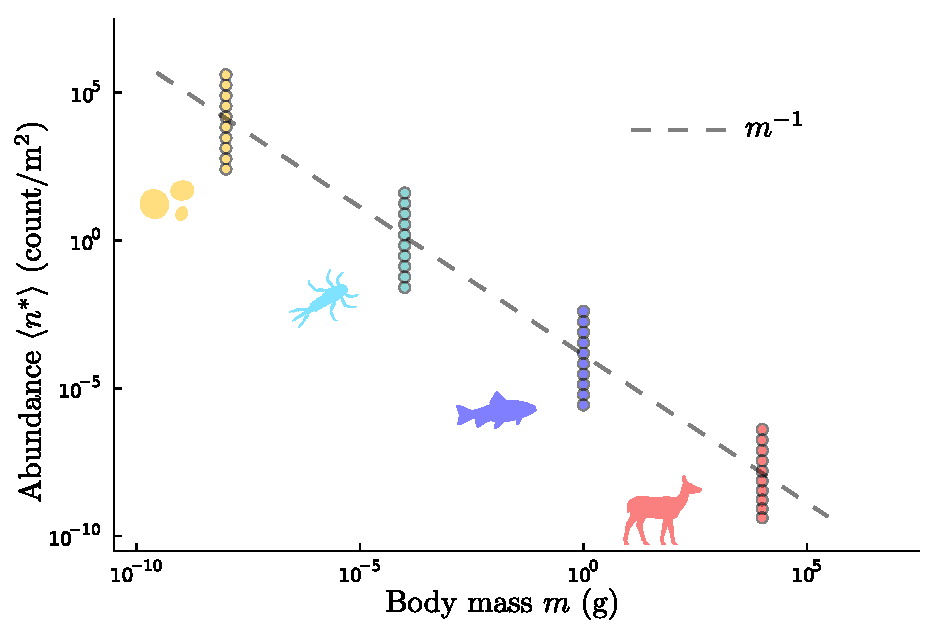
\includegraphics[width=.8\textwidth]{fig/SM-size-density-scaling.pdf}
    \caption{\textcolor{red}{Make figure with precise values of r} Numerical density distribution vs. body mass for each community 
     type parametrized as in the model construction (Fig.~\ref{fig: SM production}).}
    \label{fig: SM size-density scaling}
\end{figure}

\section{Macroecology with GLV}
In this section we discuss how to reproduce the production data
wiht the GLV model and under what assumption it recovers the macroecological
pattern discussed in the paper.

Let us recall the GLV model to describe the 
biomass density of S species
\begin{equation}
    \frac{d B_i}{dt} = r_iB_i\left(1-\frac{B_i}{K_i}\right) - \sum_{j\neq i}A_{ij}B_j \, ,
\end{equation}
where $A_{ij}$ are distributed with mean $\mu$ and standard deviation $\sigma$, 
$K_i$ are the carrying capicties and we redefine the growth rates $r_i$
as the difference between growht and mortality rate defined before, i.e.
$\bar{r}_i:=r_i-z_i$ and we drop the bar.
The cavity solution for this system reads~\cite{Bunin2017}
\begin{equation}
    B^* = K\left(1 - \frac{\mu S\langle B^*\rangle +
    \sigma\sqrt{S\langle (B^*)^2\rangle}}{r}\right) \, ,
    \label{eq: SM cavity GLV}
\end{equation}
with $r$ and $K$ in general distributed as $P(r)$ and $P(K)$
respectively.

Let us work in the case in which $r$ and $K$ are the same for every speceis 
and we assume $\sigma\to 0$ for simplicity to discuss the assumption
needed to obtain the production scaling. In this case 
each species in the community has the same biomass density
\begin{equation}
    B^* = \frac{K}{1+\mu S K/r} \, ,
\end{equation}
which recovers $B^* = K$ for vanishing inter-species interactions.

We will assume that intra-specific and inter-specific 
interactions scale in the same way $\mu = a  r / K$ 
(with $a<1$ to guarantee sabitlity).
Notice that for $a\simeq1$, for large $S$, we can write
$B^* \simeq K/S$,
which allows for an intrepretation of $K$
as a community parameter, a global carrying capacity, 
which encode the maximum biomass density that a specific ecosystem can
sustain. In the following we arbitrarly set $a=1/S$ in order
to have good stability properties, in this case $B^*=K/2$. 

\subsection{Production-biomass scaling}
The key assumption we need to connect with sublinear proiduciton-biomass 
scaling is that the growth rate $r$ should scale with the carrying capacity as
$r=bK^{k-1}$.
The production, using the solution for $B^*$ and our assumptions reads then
\begin{equation}
    rB^*\left(1-\frac{B^*}{K}\right) = \frac{b}{2^{2-k}}(B^*)^{k} \, .
    \label{eq: SM analytic production GLV}
\end{equation}
As we show in Fig.~\ref{fig: SM production GLV} this result holds also
for finite $\sigma$ (we set $\sigma=\mu$).

In order to reproduce the data, we set for each community $b$
as the difference of the representative growth rates 
and mortalities discussed in the
main text, namely 0.37 for mammal, 7.05 for fish, 30 for invertebrate
and 437 for protists. 
Then a variation of 4 order of magnitude for $K$ is consistent with
1 order of magnitude variation around these values for the effective growth rates.
In Fig.~\ref{fig: SM production GLV} we report comparisons of simulations
with analytical prediction of the produciton-biomass scaling.

\begin{figure}[h!]
    \centering
    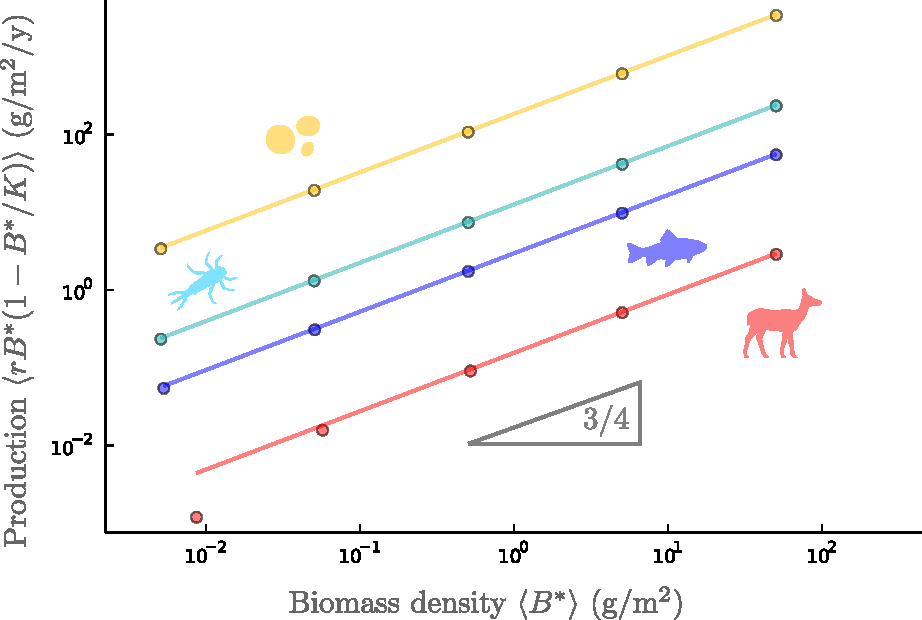
\includegraphics[width=.8\textwidth]{fig/SM-production-GLV.pdf}
    \caption{Average equilibrium production 
    plotted versus average equilibrium biomass density.
    Each dot represents simulations for a community of $S=50$ species, 
    each color correspond to a specific difference between growth and mortality
    value: $437$ yellow, $30$ light blue,
    $7.05$ blue and $0.37$. The carrying capacity $K$
    is varied between $10^{-2}$ to $10^2$ and we set 
    the coefficient of variation $\sigma/\mu=1$.
    The lines represent theoretical predictions from the
    cavity solution in Eq~(\ref{eq: SM analytic production GLV}).}
    \label{fig: SM production GLV}
\end{figure}

\subsection{Macroecological patterns}
We study here predictions and consistency checks of macroecological patterns
for GLV under the assumptions 
used to recover production-biomass scaling.

\subsubsection{Species abundance distribution}
Consider a community with $r$ extracted from a log-normal
distribution, $\ln{r}\sim\mathcal{N}(\mu_r, \sigma_r)$,
and for simplicity we cosnider $\sigma\to 0$.
The cavity solution reads
\begin{equation}
    B^* = K - \frac{\mu S K\langle B^*\rangle}{r} \, .
\end{equation}
Following our assumptions $K=(r/b)^{1/(k-1)}$ and we have
\begin{equation}
    B^* = (r/b)^{1/(k-1)} - \langle B^*\rangle \, ,
\end{equation}
therefore we have that, defining $\bar{B}^*:=B^*+\langle B^*\rangle$,
\begin{equation}
    \ln{\bar{B}^*} \sim \mathcal{N}(\mu_{\bar{B}^*},\sigma_{\bar{B}^*}) \, ,
\end{equation}
with
\begin{equation}
    \mu_{\bar{B}^*} = \frac{\ln{b}-\mu_r}{1-k} \, ,
\end{equation}
and
\begin{equation}
    \sigma_{\bar{B}^*} = \frac{\sigma_r}{1-k} \, .
\end{equation}
Therefore, as in the case of the sublinear model, 
we obtain a distribution 
for $B^*$ four times wider than the one for $r$
when $k=3/4$. 

\subsubsection{Mean-variance scaling}
In order to study the mean-variance scaling, 
we consider the variance of $B^*$ which,
from Eq.~(\ref{eq: SM cavity GLV}), reads
\begin{equation}
    \langle (B^*)^2 \rangle - \langle B^* \rangle^2 = 
    \frac{\sigma^2K^2S\langle (B^*)^2\rangle}{r^2} \, .
\end{equation}
Following our assumption we have $\sigma=\mu =r /KS$ and 
therefore we conclude that
\begin{equation}
    \textrm{var}(B^*) = \frac{\langle B^* \rangle^2}{S-1} \, .
\end{equation}

\subsubsection{Size-denisty scaling}
Consistency with the size-density scaling is straightforward
because within our assumption $B^*$ does not depend
on $r$, i.e. on the community type and ultimately on $m$.
We have therefore
\begin{equation}
    N^* = \frac{B^*}{m} \propto m^{-1} \, .
\end{equation}

\newpage

\section{Back up sections}

\subsection{Generalized Lotka-Volterra with generic production}
\textcolor{red}{Maybe take out.}

Consider a competitive community of $S$ species
defined by the following dynamics for the population abundances
\begin{equation}
    \frac{dx_i}{dt}=g(x_i)-x_i\sum_{j\neq i}A_{ij}x_j \, ,
\end{equation}
where the $A_{ij}$ are extracted from a distribution
with mean $\mu>0$ and standard deviation $\sigma$ and
the production term $g_i(x_i)$ may in principle include
self-regulation terms which are only dependent on species $i$
and parameters typical of species $i$.

If the equilibrium is feasible, denoting $x_i^*$ the equilibrium values,
we have
\begin{equation}
    g_i(x_i^*)=x_i^*\sum_{j\neq i}A_{ij}x_j^* \, .
\end{equation}
The jacobian evaluated at equilibrium is formally
\begin{equation}
    J_{ij}\Big{|}_{\bf{x}=\bf{x}^*} = -x_i^*A_{ij} \, ,
\end{equation}
\begin{equation}
    J_{ii}\Big{|}_{\bf{x}=\bf{x}^*} =  g_i'(x_i^*)-\frac{g_i(x_i^*)}{x_i^*}\, ,
\end{equation}
where $g_i'(x_i^*)$ stands for $|d g_i(x_i)/d x_i|_{x_i=x_i^*}$ 
and we used the equilibrium relation.

In order to make some analytical progress let us focus on the case
of uniform interactions ($\sigma\to0$) and production
with same parameters for every species, i.e. $g_i=g$ $\forall i$.
Then every species have the same equilibrium value $x_i^*=x^*$
$\forall i$ and we can write down the equilibrium relation
\begin{equation}
    g(x^*)=(S-1)\mu (x^*)^2 \, ,
\end{equation}
and the jacobian at equilibrium
\begin{equation}
    J_{ij}\Big{|}_{x=x^*} = -x^*\mu \, ,
\end{equation}
\begin{equation}
    J_{ii}\Big{|}_{x=x^*} =  g'(x^*)-\frac{g(x^*)}{x^*}\, .
\end{equation}
The largest eigenvalue correspond to
\begin{equation}
    \lambda_{\max}=J_{ii}\Big{|}_{x=x^*}-J_{ij}\Big{|}_{x=x^*} \, ,
\end{equation}
therefore the stability condition reads
\begin{equation}
    g'(x^*)- \frac{g(x^*)}{x^*} + x^*\mu < 0 \, .
\end{equation}
By exploiting the equilibrium relation we can recast the last
inequality as
\begin{equation}
    g'(x^*)- \frac{g(x^*)}{x^*} + \frac{g(x^*)}{x^*(S-1)} < 0 \, ,
\end{equation}
therefore giving the general formal stability condition in terms
of production at equilibrium and equilibrium density
\begin{equation}
    g'(x^*) < \frac{g(x^*)}{x^*}\left(1 - \frac{1}{S-1}\right) \, ,
\end{equation}
which for $S\to\infty$ can be approximated by 
\begin{equation}
    g'(x^*) < \frac{g(x^*)}{x^*} \, .
\end{equation}
This last stability condition is quite general and, exploiting the trivial identity
$1=dx/dx|_{x=x^*}=:(x^*)'$, it can be written as
\begin{equation}
    \frac{g'(x^*)}{g(x^*)} < \frac{(x^*)'}{x^*}\, ,
\end{equation}
which means that the relative change in growth should be less than the relative
change in abundance itself.

Logistic and sublinear cases are recovered by substitutig resepctively
$g(x)=x(1-x/K)$ and $g(x)=x^k$.

\newpage

\bibliography{library.bib}

\bibliographystyle{unsrt}

\end{document}